\newcommand{\companyname}{\mbox{<<Техартгруп>>}}

\section{Охрана труда}

\subsection[Обеспечение пожарной безопасности на предприятии]{Обеспечение пожарной безопасности на предприятии малого бизнеса \companyname{}}


Целью дипломного проекта является реализация и анализ алгоритмов построения вероятностных сетей.
Вероятностная сеть является компактным и эффективным способом представления знаний.
Вероятностные сети используются в программном обеспечении для принятия решения в условиях недостаточной определенности.
Данный способ статистического моделирования показал свою пригодность в реальных условиях в сложных предметных областях: медицине, космической промышленности, финансовой сфере и других областях.
Первоначальные стадии разработки дипломного проекта выполнялись на предприятии ООО~\companyname{} во время прохождения преддипломной практики.
В настоящем разделе рассматриваются вопросы, связанные с обеспечением пожарной безопасности на предприятии.

Предприятие \companyname{} занимается предоставлением услуг по разработке информационных систем для иностранных предприятий. 
В минском офисе компании на данный момент работает более 200 человек. 
% TODO: Переписать абсолютный бред в оставшейся части абзаца.
Большое количество конкурирующих компаний, разрабатывающих программное обеспечение в Минске, способствует повышению общего уровня условий труда.
Это, в частности, сказывается на комфортабельности рабочих мест.
Работникам предоставляются светлые, проветриваемые, тихие кабинеты, гибкий график рабочего времени, специальные комнаты отдыха и т.\,д.
Современные компании негласно ориентируются на соответствие лучшим мировым практикам в области охраны труда и, в частности, пожарной безопасности.

На предприятии \companyname{} за пожарную безопасность отвечает директор компании.
Для каждого нового сотрудника производится инструктаж по пожарной безопасности и технике безопасности, а так же знакомство с планом эвакуации при возникновении черезвычайных ситуаций~\cite[\ignore{раздел~5.5.8,} с.~324]{michnuk_2009}.
За проведение инструктажа отвечает специальный человек из отдела материально"=технического снабжения предприятия.
В компании действует набор правил, обязательных для исполнения сотрудниками.
В целях повышения пожарной безопасности курение в здании офиса запрещено.
Все сотрудники обязаны в конце рабочего дня выключить свои персональные компьютеры и обесточить их.
В конце рабочего дня специальный сотрудник проверяет соблюдение данного правила в каждом рабочем кабинете, чтобы там были выключены все электрические приборы: компьютеры, электрические чайники, кондиционеры, освещение и т.\,д.
Все рабочие компьютеры подключены к источникам бесперебойного питания, которые подключены к сетевыми фильтрам, защищающим от скачков напряжения в электросети.

Офис компании расположен в центре города.
Здание офиса представляет собой монолитную железобетонную конструкцию высотой шесть этажей, офис компании находится на двух верхних этажах.
Конструкция здания предусматривает три способа эвакуации с этажа: выход в паркинг, лестничная клетка с выходом на улицу, лестничная клетка с выходом на первый этаж паркинга. 
В случае недоступности основных эвакуационных выходов из каждого кабинета можно через окно попасть на лоджию~\cite[\ignore{раздел~5.5.4,} с.~314\,--\,316]{michnuk_2009}.
Схемы эвакуации выдаются в виде электронного документа каждому новому сотруднику, а также находятся на специальном стенде в рабочих кабинетах.
Все кабинеты офиса расположены вдоль длинного коридора, который оборудован специальными аварийными светильниками и знаками, указывающими направление эвакуации.
На случай отключения электроэнергии компания имеет два дизельных"=генератора, обеспечивающих нужды предприятия на случай отключения электроэнергии.

Офис компании оборудован необходимыми средствами сигнализации о пожаре~\cite[с.~215]{sinilov_2010}. %\cite[с.~5\,--\,7]{sharovar_1979}. 
Каждый кабинет оборудован пожарным дымовым оптико"=электрическим точечным извещателем \mbox{ИП212-02М1} (рисунок~\ref{fig:fire_alarms}).
На предприятии производиться регулярный контроль и проверка работоспособности пожарных извещателей специальным человеком из отдела материально"=технического снабжения предприятия.
В коридорах дополнительно установлены ручные пожарные извещатели \mbox{ИП 5-2Р} (рисунок~\ref{fig:fire_alarms}).
Для извещения о пожаре также может быть использована корпоративная электронная почта, а также другие современные способы обмена информацией.

\begin{figure}[ht]
\centering
  \begin{subfigure}[b]{0.45\textwidth} 
    \centering
    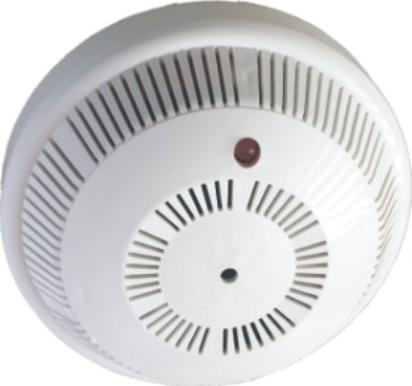
\includegraphics[scale=0.85]{avt_pozh_izv.jpg}  
    \caption{}
  \end{subfigure}
  \begin{subfigure}[b]{0.45\textwidth} 
    \centering
    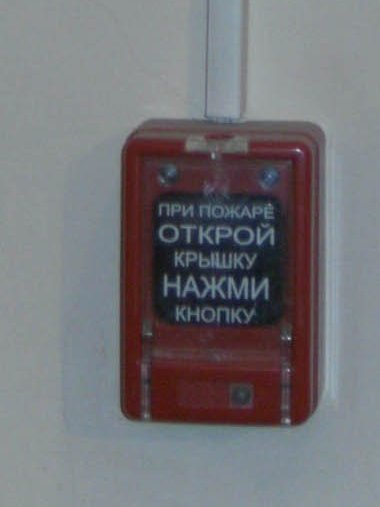
\includegraphics[scale=1.2]{ruch_pozh_izv.jpg}  
    \caption{}
  \end{subfigure}
  \caption{ а "--- автономный пожарный извещатель;
            б "--- ручной пожарный извещатель.}
  \label{fig:fire_alarms}
\end{figure}

На случай возникновения пожара в каждом рабочем кабинете находиться ручной порошковый огнетушитель \mbox{ОП-10}~(з)~МИГ~М (рисунок~\ref{fig:extinguishing_fire}), пригодный для тушения пожаров различного типа, в том числе для тушения электрических приборов~\cite[\ignore{раздел 5.5.7,} с.~221\,--\,323]{michnuk_2009}.
Каждый этаж здания офиса оборудован двумя пожарными кранами для тушения пожара.
Пожарные краны расположены в противоположных частях коридора, недалеко от эвакуационных выходов (рисунок~\ref{fig:extinguishing_fire}).
На случай воспламенения электрической проводки или другого электрического оборудования в каждом кабинете установлены электрические щитки, необходимые для отключения подачи электроэнергии в пределах кабинета.
Во всех помещениях офиса предприятия установлена оросительная система пожаротушения для ликвидации возгорания до приезда пожарной службы~\cite[\ignore{раздел~5.5.6,} с.~318\,--\,320]{michnuk_2009}.
При расследовании возможных причин возникновения пожара может быть задействована система видео"=наблюдения, установленная во всех помещениях предприятия.

\begin{figure}[ht]
\centering
  \begin{subfigure}[b]{0.45\textwidth} 
    \centering
    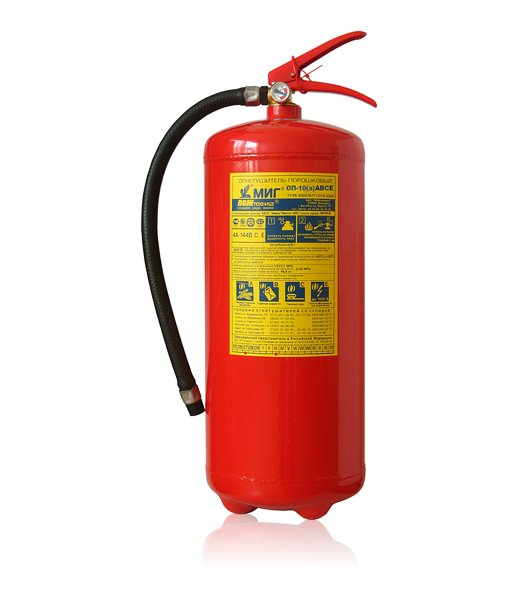
\includegraphics[scale=0.34]{ognetush.jpg}  
    \caption{}
  \end{subfigure}
  \begin{subfigure}[b]{0.45\textwidth} 
    \centering
    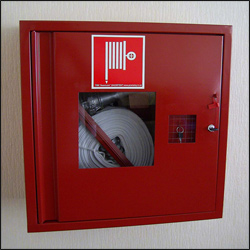
\includegraphics[scale=0.7]{pozh_kran.jpg}  
    \caption{}
  \end{subfigure}
  \caption{ а "--- порошковый огнетушитель \mbox{ОП-10}~(з)~МИГ~М;
            б "--- пожарный кран.}
  \label{fig:extinguishing_fire}
\end{figure}

Основной род деятельности на предприятии "--- разработка информационных систем "--- не предусматривает непосредственный контакт с горючими или легко"=воспламеняющимися веществами, что сильно снижает риски возникновения пожара на предприятии.
Наиболее вероятными причинами возникновения пожара, с учетом специфики предприятия, могут являться нарушение правил внутреннего распорядка "--- курение на рабочем месте, и неисправность электрического оборудования, которого в офисе компании достаточно~\cite[\ignore{раздел 5.5.1,} с.~312]{michnuk_2009}.
С целью снижения риска возникновения пожара по причине неисправности электрического оборудования в компании запрещено пользоваться неисправным оборудованием, а все исправное оборудование подключается в сеть через специальные сетевые фильтры и источники бесперебойного питания.
В целом правила распорядка на предприятии и высокая культура работы с электрическим оборудованием снижают риски возникновения пожара до минимума.

Большой проблемой в достижении максимальной пожарной безопасности предприятия является доступность подъезда пожарной техники к зданию офиса.
В будние дни прилегающие улицы, стоянки, пешеходные переходы заняты неправильно припаркованным личным транспортом.
Большую часть светлого времени суток движение по прилегающим улицам очень затруднено.
Данную проблему предприятие не в силах решить самостоятельно, проблема заключается в низкой культуре владельцев транспорта и игнорировании многочисленных нарушений правил дорожного движения  сотрудниками ГАИ.
% Заключительное предложение
Таким образом, изложенные выше предложения, не смотря на проблемы с подъездом пожарной техники, обеспечат пожарную безопасность на предприятии \companyname{}.
